\section{MLCommons Medical AI}
{{\footnotesize
\begin{description}[labelwidth=5em, labelsep=1em, leftmargin=*, align=left, itemsep=0.3em, parsep=0em]
  \item[date:] 2023-07-17
  \item[version:] TODO
  \item[last\_updated:] 2023-07
  \item[expired:] unknown
  \item[valid:] yes
  \item[valid\_date:] TODO
  \item[url:] \href{https://github.com/mlcommons/medical}{https://github.com/mlcommons/medical}
  \item[doi:] TODO
  \item[domain:] Healthcare; Medical AI
  \item[focus:] Federated benchmarking and evaluation of medical AI models across diverse real-world clinical data
  \item[keywords:]
    - medical AI
    - federated evaluation
    - privacy-preserving
    - fairness
    - healthcare benchmarks
  \item[summary:] The MLCommons Medical AI working group develops benchmarks, best practices, and platforms (MedPerf, GaNDLF, COFE)
to accelerate robust, privacy-preserving AI development for healthcare. MedPerf enables federated testing of clinical
models on diverse datasets, improving generalizability and equity while keeping data onsite :contentReference[oaicite:1]\{index=1\}.

  \item[licensing:] TODO
  \item[task\_types:]
    - Federated evaluation
    - Model validation
  \item[ai\_capability\_measured:]
    - Clinical accuracy
    - fairness
    - generalizability
    - privacy compliance
  \item[metrics:]
    - ROC AUC
    - Accuracy
    - Fairness metrics
  \item[models:]
    - MedPerf-validated CNNs
    - GaNDLF workflows
  \item[ml\_motif:]
    - Multiple
  \item[type:] Platform
  \item[ml\_task:]
    - NA
  \item[solutions:] TODO
  \item[notes:] Open-source platform under Apache-2.0; used across 20+ institutions and hospitals :contentReference[oaicite:2]\{index=2\}.

  \item[contact.name:] Alex Karargyris (MLCommons Medical AI)
  \item[contact.email:] unknown
  \item[datasets.links.name:] Multi-institutional clinical datasets, radiology
  \item[results.links.name:] ChatGPT LLM
  \item[fair.reproducible:] Yes
  \item[fair.benchmark\_ready:] Yes
  \item[ratings.software.rating:] 0
  \item[ratings.software.reason:] Not analyzed.

  \item[ratings.specification.rating:] 9.0
  \item[ratings.specification.reason:] Diverse scientific tasks (earthquake, CFD, microscopy) with detailed problem statements and goals; system constraints not uniformly applied.

  \item[ratings.dataset.rating:] 9.0
  \item[ratings.dataset.reason:] Domain-specific datasets (e.g., microscopy, climate); mostly public and structured, but FAIR annotations are not always explicit.

  \item[ratings.metrics.rating:] 9.0
  \item[ratings.metrics.reason:] Task-specific metrics (MAE, speedup, accuracy) are clear and reproducible.

  \item[ratings.reference\_solution.rating:] 9.0
  \item[ratings.reference\_solution.reason:] Reference models (CNN, GNN, Transformer) provided with training/evaluation pipelines.

  \item[ratings.documentation.rating:] 9.0
  \item[ratings.documentation.reason:] Well-documented, open-sourced, and maintained with examples; strong community support and reproducibility focus.

  \item[id:] mlcommons\_medical\_ai
  \item[Citations:] \cite{karargyris2023federated}
  \item[Ratings:]
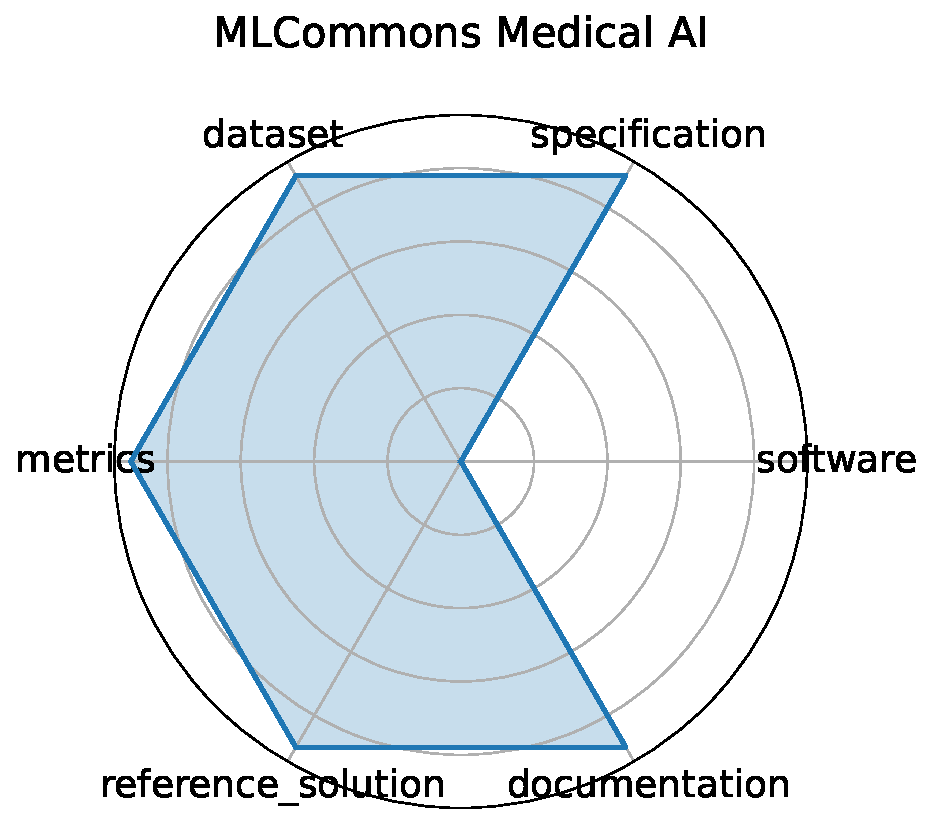
\includegraphics[width=0.2\textwidth]{mlcommons_medical_ai_radar.pdf}
\end{description}
}}
\clearpage